%
% $XORP: xorp/docs/mfea/mfea_arch.tex,v 1.8 2003/06/09 20:02:21 pavlin Exp $
%

\documentclass[11pt]{article}

%\usepackage[dvips]{changebar}

\usepackage{subfigure}
\usepackage{fullpage}
\usepackage{setspace}
\usepackage{times}
\usepackage{latexsym}
\usepackage{psfig}
\usepackage{graphicx}
\usepackage{xspace}
\usepackage{color}
\usepackage{amsmath}
%\usepackage[dvipdf]{graphics}
%\usepackage[dvips]{graphicx}
%\usepackage{xorp}

\definecolor{gray}{rgb}{0.5,0.5,0.5}
\newcommand{\etc}{\emph{etc.}\xspace}
\newcommand{\ie}{\emph{i.e.,}\xspace}
\newcommand{\eg}{\emph{e.g.,}\xspace}
%\newcommand{\comment}[1]{{\color{gray}[\textsf{#1}]}}
\newcommand{\comment}[1]{}

% Changebar stuff
% \newenvironment{colorcode}{\color{blue}}{}
% \renewcommand{\cbstart}{\begin{colorcode}}
% \renewcommand{\cbend}{\end{colorcode}}

% \pagestyle{empty}

\begin{document}

\title{XORP Multicast Forwarding Engine Abstraction \\
\vspace{1ex}
Version 0.4}
\author{ XORP Project					\\
	 International Computer Science Institute	\\
	 Berkeley, CA 94704, USA			\\
	 {\it feedback@xorp.org}
}
\date{August 28, 2003}

\maketitle

\thispagestyle{empty}


%%%%%%%%%%%%%%%%%%%%%%%%%%%%%%%%%%%%%%%%%%%%%%%%%%%%%%%%%%%%%%%%%%%%%%%
\section{Introduction}


%%%%%%%%%%%%%%%%%%%%%%%%%%%%%%%%%%%%%%%%%%%
\subsection{Overview}

This document provides an overview of the XORP Multicast Forwarding
Engine Abstraction (MFEA). It is intended to provide a starting point
for software developers who wish to modify this software.

The main purpose of the MFEA is to abstract the underlying system and
the multicast forwarding engine, and to provide a consistent interface
to multicast-related modules such as PIM and MLD/IGMP. Thus, if we want
to use PIM and MLD/IGMP on different OS platform or hardware, we
would have to modify the MFEA only. In addition, all the
complexity associated with network sockets, sending and receiving
packets, and so on are moved away from the protocol modules.
This eliminates code duplication, and reduces greatly the
development overhead associated with protocol-independent
issues when implementing a new protocol. Finally, if we want to use
PIM and MLD/IGMP in a simulation-like environment, it will be sufficient
to add the simulation environment support only to the MFEA.

Currently (August 2003), the MFEA supports abstraction for
the following systems:

\begin{itemize}
  \item \{Free,Net,Open\}BSD OS (tested only on FreeBSD-4.5 and FreeBSD-4.7).
  \item Linux OS (tested only on Red Hat Linux 7.2 with kernel 2.4.18)
\end{itemize}

In the future, the MFEA will support simulation environment, and
abstraction for Click~\cite{CLICK-PROJECT} forwarding
path~\footnote{Currently (August 2003) Click does
not support multicast yet.}. Support for other systems will be added
on-demand if there are available resources.

Note that typically the MFEA would be part of the unicast FEA
process~\cite{xorp:fea}, though logically it is a separate entity.
However, if someone wants to run the MFEA as a separate process, it
requires very small development effort to do this because of the logical
separation between the FEA and the MFEA.

%%%%%%%%%%%%%%%%%%%%%%%%%%%%%%%%%%%%%%%%%%%
\subsection{Acronyms}

Acronyms used in this document:

\begin{itemize}

  \item {\bf FEA}: {\bf F}orwarding {\bf E}ngine {\bf A}bstraction

  \item {\bf MFC}: {\bf M}ulticast {\bf F}orwarding {\bf C}ache: another
  name for an entry in the multicast forwarding engine (typically used
  on UNIX systems).

  \item {\bf MFEA}: {\bf M}ulticast {\bf F}orwarding {\bf E}ngine
  {\bf A}bstraction

  \item {\bf MLD/IGMP}: {\bf M}ulticast {\bf L}istener {\bf D}iscovery/{\bf
  I}nternet {\bf G}roup {\bf M}anagement {\bf P}rotocol

  \item {\bf MRIB}: {\bf M}ulticast {\bf R}outing {\bf I}nformation
  {\bf B}ase

  \item {\bf PIM-SM}: {\bf P}rotocol {\bf I}ndependent {\bf M}ulticast--{\bf
  S}parse {\bf M}ode

  \item {\bf RIB}: {\bf R}outing {\bf I}nformation {\bf B}ase

\end{itemize}


%%%%%%%%%%%%%%%%%%%%%%%%%%%%%%%%%%%%%%%%%%%
\subsection{MFEA Design Architecture Overview}

\begin{figure}[htbp]
  \begin{center}
    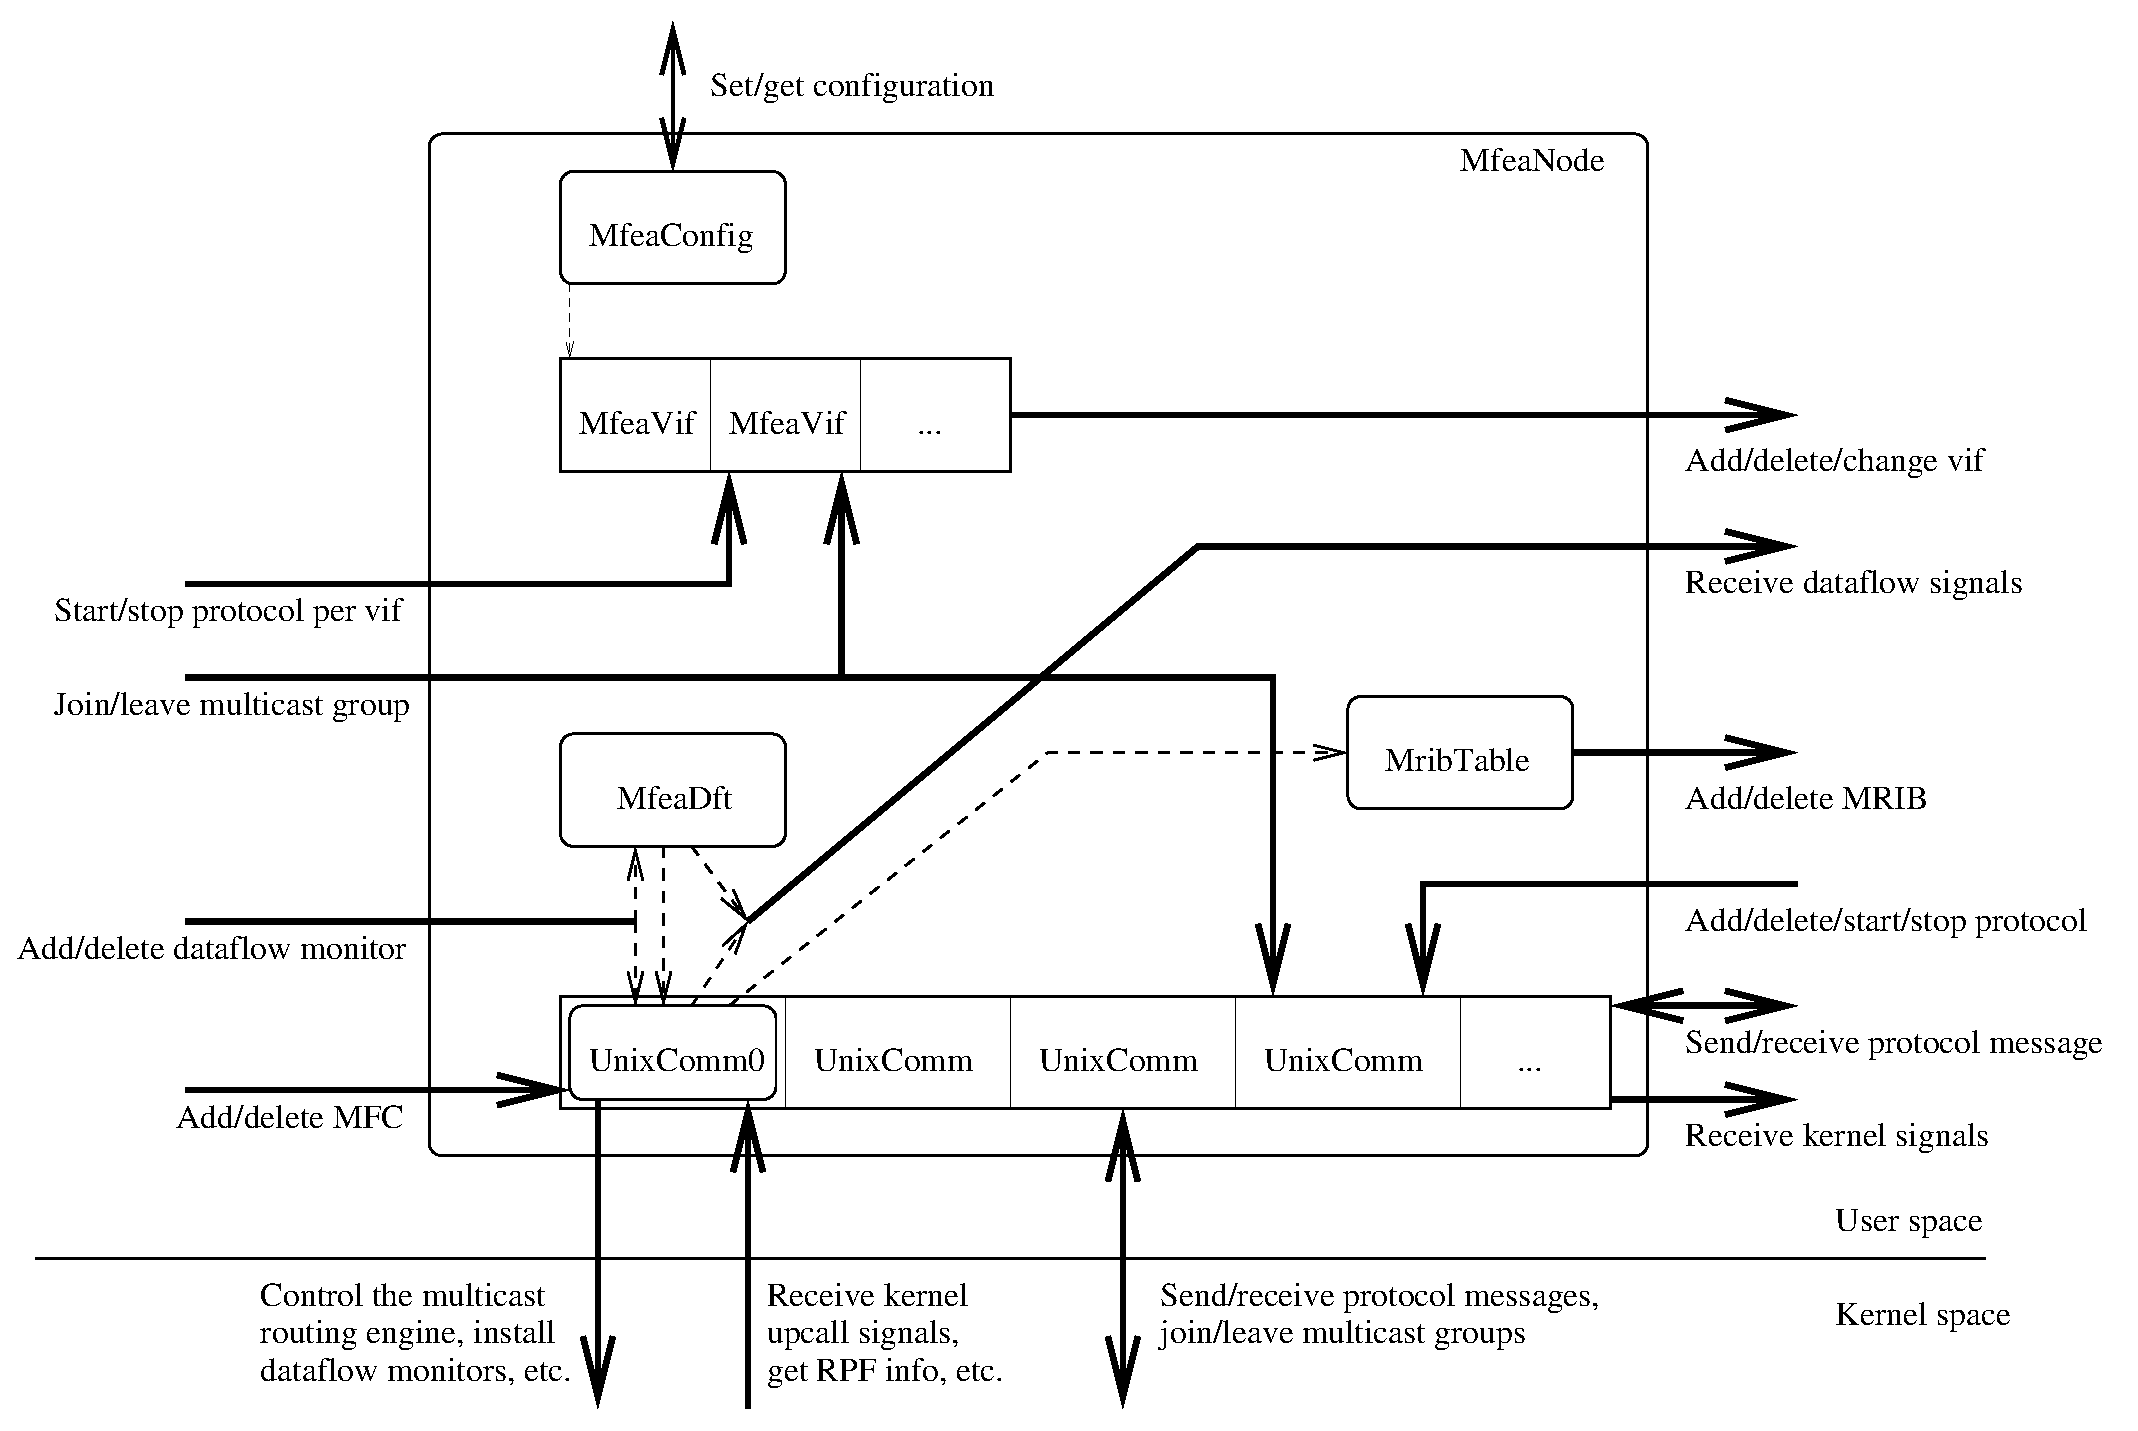
\includegraphics[scale=0.5]{figs/mfea_design_overview}
    \caption{MFEA design overview}
    \label{fig:mfea_design_overview}
  \end{center}
\end{figure}

Figure~\ref{fig:mfea_design_overview} provides a general overview of the
MFEA components. For each component there is a C++ class with exactly
the same name. The main components are briefly described below:

\begin{itemize}

  \item {\bf MfeaNode:} a representation of a single MFEA unit
  (\eg as part of a virtual multicast router).
  Typically, there would be a single MfeaNode per multicast router.

  \item {\bf MfeaVif:} MFEA-specific virtual (network) interface that is used
  to keep state per network interface.

  \item {\bf MfeaConfig:} contains MFEA-specific configuration.

  \item {\bf MfeaDft:} table with dataflow-related information for
  estimating the bandwidth per dataflow.

  \item {\bf MribTable:} the table with MRIB information.

  \item {\bf ProtoComm:} per-protocol UNIX-specific unit for
  communication with the underlying system.

  \item {\bf MfeaMrouter:} unit for multicast-related communication with
  the underlying system.

\end{itemize}

Those components are described in details in
Section~\ref{sec:components_description}.
For information about the interaction between the MFEA and other modules see
\cite{xorp:multicast_arch}.

%%%%%%%%%%%%%%%%%%%%%%%%%%%%%%%%%%%%%%%%%%%%%%%%%%%%%%%%%%%%%%%%%%%%%%%
\section{Components Description}
\label{sec:components_description}


%%%%%%%%%%%%%%%%%%%%%%%%%%%%%%%%%%%%%%%%%%%
\subsection{MfeaNode Description}

MfeaNode is a representation of a single MFEA unit (\eg as part of a
virtual multicast router).
Typically, there would be a single MfeaNode per multicast router.
However, in some cases a multicast router may have more than one
MFEA units. For example, it could have one MfeaNode for IPv4, and
another one for IPv6 multicast routing. Further, if we want to
run MFEA in a simulation environment, each multicast router within that
simulation will have a single MfeaNode.

From a developer's point of view, MfeaNode contains all the state
related to the MFEA unit, and exports the front-end interface
to interact with that unit.
For example, MfeaNode contains the methods to
start/stop or configure the MFEA, or to send/receive protocol control
packets (\eg PIM or MLD/IGMP) to/from the unit. Those methods are
described in the following files:

\begin{itemize}
  \item \verb=mfea/mfea_node.hh=
  \item \verb=libproto/proto_node.hh=
  \item \verb=libproto/proto_unit.hh=
\end{itemize}

MfeaNode provides the following abstraction to the multicast-related
modules such as PIM and MLD/IGMP:

\begin{itemize}

  \item Interface to add/delete/start/stop a protocol within the MFEA
  and the underlying system.

  \item Interface to send or receive protocol packets through the
  underlying system.

  \item Interface to receive (kernel) upcalls/signals from the
  underlying system, and to forward those signals to the
  multicast-related modules that are interested in receiving those
  signals. Examples of such signals in case of UNIX kernel are NOCACHE or
  WRONGVIF/WRONGMIF: the former one is sent when the underlying multicast
  forwarding engine has no multicast forwarding entry for a multicast
  packet; the latter one is sent when a multicast data packet has
  arrived on an interface that is not the expected incoming interface to
  forward that data packet.

  \item Interface to add/delete dataflow monitors, to monitor network
  bandwidth per dataflow, and to send the appropriate signals to the
  interested multicast-related modules. For example, the PIM-SM module
  might be interested to know when the bandwidth of a given dataflow becomes
  zero, or is above a threshold.

  \item Interface to inform the multicast-related modules about the
  available virtual interfaces (\eg network interfaces, tunnels, etc.) on
  the system, and to inform them about any changes on those interfaces
  (\eg interface going DOWN, network address change, etc.).

  \item Interface to join or leave a multicast group.

  \item Interface to add/delete MFC entries, \ie entries to the
  multicast forwarding engine.

  \item Interface to send the MRIB information to the interested
  multicast-related modules. Note that this is a temporary solution, and
  in the future (after August 2003) the multicast modules interested in
  the MRIB will obtain this information from the RIB module instead.

\end{itemize}

MfeaNode itself does not implement the mechanisms to communicate with
the multicast-related modules (\eg to send or receive control packets
to/from the PIM module). Those mechanisms are outside the scope of
MfeaNode, and must be implemented separately.

MfeaNode contains several pure virtual methods (\eg
\verb=send_add_mrib()= is used to add MRIB entry to a
multicast-related module that is interested in tracking the MRIB) 
that must be implemented by a class that inherits MfeaNode.
For example, XrlMfeaNode is a class that uses MfeaNode as a base class;
XrlMfeaNode uses XRL-based communication mechanisms between MfeaNode
and other XORP components such as the PIM and MLD/IGMP modules.

By default, MfeaNode is disabled; therefore, on startup it must be
enabled explicitly.

%%%%%%%%%%%%%%%%%%%%%%%%%%%%%%%%%%%%%%%%%%%
\subsection{MfeaVif Description}

MfeaVif is a MFEA-specific virtual (network) interface that is used to keep
various state per interface. Typically, there would be one
MfeaVif per network interface such as physical
interface, tunnel, or the loopback interface. In addition, there is
one special MfeaVif: the PIM Register virtual
interface that is used for sending and receiving PIM Register
packets~\footnote{In the future (after August 2003), the PIM
Register MfeaVif interface may not be part of the MFEA anymore, because
it is strictly PIM-specific.}.

One of the purposes of MfeaVif is to keep various information about each
network interface available on the system: network and subnet address,
is the interface up or multicast-capable, and so on. This information is
obtained from the FEA (the only exception is the PIM Register vif which
is created internally by the MFEA), and is used by the MFEA to keep
track of any changes to an interface (\eg an alias address has been
added/deleted, etc). If there is a change to an interface, those changes
are saved locally by the MFEA, and then the MFEA informs all protocol
modules that are registered by the MFEA.

Another purpose of MfeaVif is to keep track of the multicast groups that
have been joined per interface. For example, if a multicast-related
module that uses the MFEA joins a multicast group on an interface, the
MFEA uses the appropriate system call to join the group on the
specified interface, and at the same time it would keep the appropriate
state on the corresponding MfeaVif. Thus, if another module joins
exactly same multicast group on that interface, but later one of
those modules leaves that group, the MFEA would modify only the appropriate
state in MfeaVif, but will not use a system call to leave the multicast
group on the interface.

Typically, from developer's point of view, all interactions with MfeaVif
would be through MfeaNode~\footnote{For simplicity, currently (August
2003) there are few occasions when XrlMfeaNode uses direct access to MfeaVif.}.

The public interface for MfeaVif contains the methods to manipulate a
virtual (network) interface. Those methods are to start/stop/enable/disable a
virtual interface, and to configure it. The methods are described in
the following files:

\begin{itemize}
  \item \verb=mfea/mfea_vif.hh=
  \item \verb=libxorp/vif.hh=
  \item \verb=libproto/proto_unit.hh=
\end{itemize}

By default, each MfeaVif is disabled; therefore, on startup it must be
enabled explicitly.


%%%%%%%%%%%%%%%%%%%%%%%%%%%%%%%%%%%%%%%%%%%
\subsection{MfeaConfig Description}

MfeaConfig handles the MFEA-specific configuration~\footnote{Currently
(August 2003), MfeaConfig is not implemented; rather, all state is
kept inside MfeaNode instead.}. This configuration is used to configure the
following units:

\begin{itemize}

  \item MfeaNode: how often to read the unicast forwarding table,
  default routing metrics and metric preferences to assign to each
  route, etc.

\end{itemize}


%%%%%%%%%%%%%%%%%%%%%%%%%%%%%%%%%%%%%%%%%%%
\subsection{MfeaDft Description}

Some protocols such as PIM-SM need the bandwidth of multicast data flows
to be monitored: if the bandwidth of a specific data flow (defined by
a source and a group address) is above or below a pre-defined threshold
(defined per data flow), the protocol should be informed. For example, if the
bandwidth of a data flow is zero for some predefined amount of time, the
corresponding multicast routing entry in the multicast routing protocol
module might be deleted (as well as the corresponding multicast
forwarding entry in the multicast forwarding engine). Another example is
the Shortest-Path Tree switch in case of PIM-SM: the SPT switch is
triggered if the bandwidth from a specific source is above a
pre-configured threshold.

If the multicast forwarding engine in the underlying system does
support bandwidth dataflow monitoring, then any addition or
deletion of a dataflow monitor to the MFEA translates to a system call
to the underlying system, and the MFEA itself does not need to keep any
state. However, if the underlying system does not support bandwidth
dataflow monitoring, then the MFEA needs to implement that on its own.
In case of UNIX kernel for example, the kernel supports an ioctl()
system call to obtain the number of octets and packets forwarded so far on
an existing MFC entry. Thus, if the MFEA reads this information twice,
it can compute the data bandwidth between the two readings.

The purpose of the MfeaDft table is to keep state about the dataflows the
MFEA is monitoring (only in the case the underlying
system does not support bandwidth dataflow monitoring). For each entry
in MfeaDft, the MFEA periodically reads the bandwidth forwarding
statistics from the underlying system. If the forwarded bandwidth
satisfies the pre-defined condition for that dataflow, the MFEA
originates a dataflow signal to the module that has installed that
dataflow monitoring entry. This signal is delivered every time the
pre-defined condition is true (until the entry is explicitly deleted by
the module that installed it).

%%%%%%%%%%%%%%%%%%%%%%%%%%%%%%%%%%%%%%%%%%%
\subsection{MribTable Description}

MribTable is the table with the MRIB information. Whenever this
information changes, the change is propagated to all interested
parties that have registered interest in it. For example, in
case of PIM-SM the MRIB is used to compute the Reverse-Path Forwarding
information toward the RPs or the senders. This information contains the
next-hop router address and the interface toward that router, the
routing metric and the metric preference.

Currently (August 2003), the MRIB information is obtained by
periodically reading the underlying unicast forwarding table by directly
calling the appropriate method in the FEA. In the
future, the MRIB would be obtained by the interested parties directly
from the RIB module instead of the MFEA module; the MFEA itself should
be used only as a backup solution, and only if explicitly enabled for
that purpose.

%%%%%%%%%%%%%%%%%%%%%%%%%%%%%%%%%%%%%%%%%%%
\subsection{ProtoComm Description}

ProtoComm is a per-protocol unit for communication with the
underlying system.

ProtoComm implements various methods that use the appropriate system
calls to open or close a socket per protocol, to send or receive
protocol packets, to join or leave a multicast group (per protocol per
interface), and so on. Typically, there is a single ProtoComm entry per
protocol; \eg one ProtoComm for PIM, another one for IGMP (or MLD in
case of IPv6), etc. When a protocol module registers a network protocol
with MFEA, the corresponding ProtoComm for that protocol is created (if
it did not exist).

Each ProtoComm entry is also used to keep information about various
protocol preferences: \eg whether a protocol module instance is interested in
receiving various kernel upcall signals, whether it needs to receive
MRIB information, etc.

%%%%%%%%%%%%%%%%%%%%%%%%%%%%%%%%%%%%%%%%%%%
\subsection{MfeaMrouter Description}

MfeaMrouter is an unit used for multicast-related communication with the
underlying system. For example, MfeaMrouter is used for the following
tasks (this list may not be complete):

\begin{itemize}

  \item Start/stop the multicast forwarding engine.

  \item Add/delete an interface used for multicast forwarding by the
  underlying system.

  \item Add/delete a MFC entry within the multicast forwarding engine.

  \item Install dataflow monitors (only if the underlying system supports
  that feature).

  \item Read data bandwidth forwarding statistics (per dataflow).

\end{itemize}

MfeaMrouter is started when MfeaNode is started, and usually stops
operation when MfeaNode is stopped.


%%%%%%%%%%%%%%%%%%%%%%%%%%%%%%%%%%%%%%%%%%%%%%%%%%%%%%%%%%%%%%%%%%%%%%%
%     APPENDIX
%%%%%%%%%%%%%%%%%%%%%%%%%%%%%%%%%%%%%%%%%%%%%%%%%%%%%%%%%%%%%%%%%%%%%%%
\appendix
\section{Modification History}

\begin{itemize}

  \item December 11, 2002: Version 0.1 completed.

  \item March 10, 2003: Updated to match XORP version 0.2 release code;
  cleanup.

  \item June 9, 2003: Updated to match XORP version 0.3 release code
  (changes related to the MFEA--FEA merging, and refactoring of
  some of the MFEA internals).

  \item August 28, 2003: Bump-up the version number to 0.4.

\end{itemize}


%%%%%%%%%%%%%%%%%%%%%%%%%%%%%%%%%%%%%%%%%%%%%%%%%%%%%%%%%%%%%%%%%%%%%%%
%     BIBLIOGRAPHY
%%%%%%%%%%%%%%%%%%%%%%%%%%%%%%%%%%%%%%%%%%%%%%%%%%%%%%%%%%%%%%%%%%%%%%%
\bibliography{../tex/xorp}
\bibliographystyle{plain}

%%%%%%%%%%%%%%%%%%%%%%%%%%%%%%%%%%%%%%%%%%%%%%%%%%%%%%%%%%%%%%%%%%%%%%%
\end{document}
